% !Mode:: "TeX:UTF-8"
% 七年级上学期第一单元几何体展开图

\begin{defproblem}{7NJ-02-01}%
\begin{onlyproblem}%
下列四个图形中,是三棱柱的表面展开图的是
\begin{center}
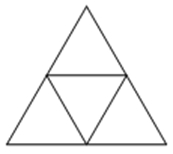
\includegraphics[width=2cm]{7NJ01-01-20190803-1.jpg}
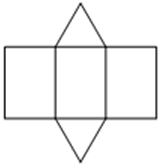
\includegraphics[width=2cm]{7NJ01-01-20190803-2.jpg}
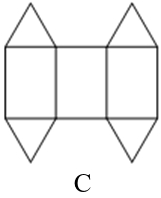
\includegraphics[width=2cm]{7NJ01-01-20190803-3.jpg}
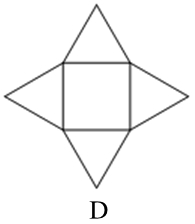
\includegraphics[width=2cm]{7NJ01-01-20190803-4.jpg}
\end{center}
\end{onlyproblem}%
\begin{onlysolution}%
\begin{solution}%%
B
\end{solution}%
\end{onlysolution}%
\end{defproblem}





\begin{defproblem}{7NJ-02-02}%
\begin{onlyproblem}%
下面6个图形是正方体的表面展开图的有
\begin{center}
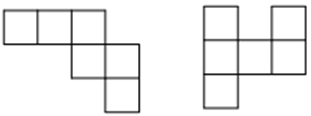
\includegraphics[width=4cm]{7NJ01-01-20190803-5.jpg}
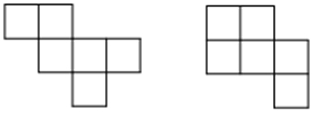
\includegraphics[width=4cm]{7NJ01-01-20190803-6.jpg}
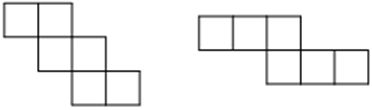
\includegraphics[width=4cm]{7NJ01-01-20190803-7.jpg}
\end{center}
\xx
{2个}
{3个}
{4个}
{5个}
\end{onlyproblem}%
\begin{onlysolution}%
\begin{solution}%%
B
\end{solution}%
\end{onlysolution}%
\end{defproblem}




\begin{defproblem}{7NJ-02-03}%
\begin{onlyproblem}%
从如图的纸板上11个无阴影的正方形中选1个(将其余10个都剪去),与图中5个有阴影的正方形折成一个正方体,不同的选法有(    ) 
\begin{center}
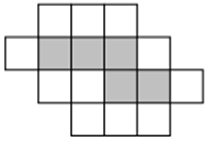
\includegraphics[width=3cm]{7NJ01-01-20190803-8.jpg}
\end{center}

\xx
{6种}
{5种}
{4种}
{3种}

\end{onlyproblem}%
\begin{onlysolution}%
\begin{solution}%%
C
\end{solution}%
\end{onlysolution}%
\end{defproblem}




\begin{defproblem}{7NJ-02-04}%
\begin{onlyproblem}%
下列四个选项的图形折叠后,能得到如图所示的正方体的是(    ) 
\begin{center}
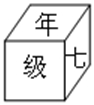
\includegraphics[width=1cm]{7NJ01-01-20190803-9.jpg}
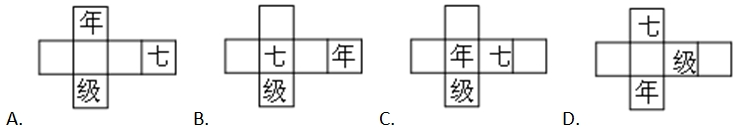
\includegraphics[width=10cm]{7NJ01-01-20190803-10.jpg}
\end{center}


\end{onlyproblem}%
\begin{onlysolution}%
\begin{solution}%%
C
\end{solution}%
\end{onlysolution}%
\end{defproblem}



\begin{defproblem}{7NJ-02-04-1}%
\begin{onlyproblem}%
如图是一个正方体纸盒的表面展开图,下列选项中的正方体能由它折叠而成的是(    ) 
\begin{center}
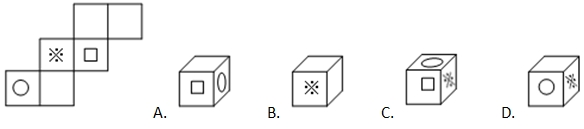
\includegraphics[width=10cm]{7NJ01-01-20190804-23}
\end{center}


\end{onlyproblem}%
\begin{onlysolution}%
\begin{solution}%%
D. 
解题思路: 根据正方体纸盒的表面展开图可知折起来之后面“$\circ$”与面“$\square$”是相对的,相对的面不可能相邻,所以折成正方体后,面“$\circ$”与面“$\square$”两个面能且只能看到一个面,排除选项A,B,C.故选D. 

\end{solution}%
\end{onlysolution}%
\end{defproblem}




\begin{defproblem}{7NJ-02-04-2}%
\begin{onlyproblem}%
如图,有一个无盖的正方体纸盒,下底面挖去了一个小洞,若沿图中粗线将其剪开展成平面图形,则这个平面图形是(    ) 
\begin{center}
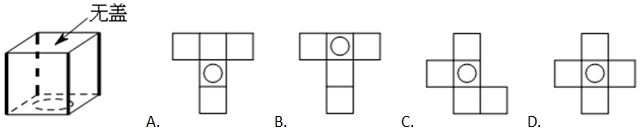
\includegraphics[width=10cm]{7NJ01-01-20190804-24}
\end{center}


\end{onlyproblem}%
\begin{onlysolution}%
\begin{solution}%%
D. 根据无盖的位置可得,面“$\circ$”展开之后没有相对面,排除B;按图中的粗线将其剪开之后与面“$\circ$”相连的四条棱均没有被剪开,排除A和C.故选D. 
\end{solution}%
\end{onlysolution}%
\end{defproblem}


\begin{defproblem}{7NJ-02-04-3}%
\begin{onlyproblem}%
下列各图都是正方体的表面展开图,若将它们折成正方体,则其中两个正方体各面图案完全一样的是(    ) 
\begin{center}
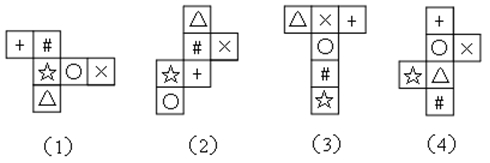
\includegraphics[width=10cm]{7NJ01-01-20190804-25}
\end{center}

\xx
{(1)(2)}
{(2)(3)}
{(3)(4)}
{(2)(4)}
  
\end{onlyproblem}%
\begin{onlysolution}%
\begin{solution}%%
选D. 
\end{solution}%
\end{onlysolution}%
\end{defproblem}



\begin{defproblem}{7NJ-02-05}%
\begin{onlyproblem}%
将“创建文明城市”六个字分别写在一个正方体的六个面上,这个正方体的表面展开图如图所示,那么在这个正方体中,和“创”相对的字是(    ) 
\begin{center}
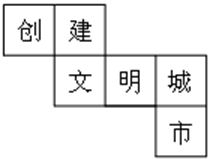
\includegraphics[width=3cm]{7NJ01-01-20190803-11.jpg}
\end{center}

\xx
{文}
{明}
{城}
{市}

\end{onlyproblem}%
\begin{onlysolution}%
\begin{solution}%%
B
\end{solution}%
\end{onlysolution}%
\end{defproblem}




\begin{defproblem}{7NJ-02-06}%
\begin{onlyproblem}%
如图,是一个正方体的表面展开图,在正方体中写有“心”字的那一面的相对面的字是(    ) 
\begin{center}
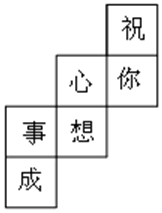
\includegraphics[width=2cm]{7NJ01-01-20190803-12.jpg}
\end{center}

\xx
{祝}
{你}
{事}
{成}

\end{onlyproblem}%
\begin{onlysolution}%
\begin{solution}%%
D
\end{solution}%
\end{onlysolution}%
\end{defproblem}



\begin{defproblem}{7NJ-02-07}%
\begin{onlyproblem}%
小明为了鼓励芦山地震灾区的学生早日走出阴影,好好学习,制作了一个正方体礼盒(如图).礼盒每个面上各有一个字,连起来组成“芦山学子加油”,其中“芦”的对面是“学”,“加”的对面是“油”,则它的表面展开图可能是(    ) 
\begin{center}
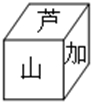
\includegraphics[width=1cm]{7NJ01-01-20190803-13.jpg}
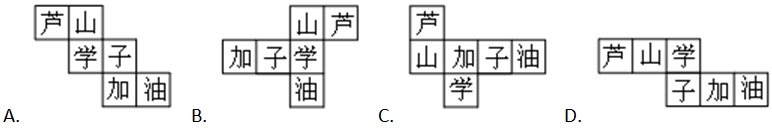
\includegraphics[width=10cm]{7NJ01-01-20190803-14.jpg}
\end{center}


\end{onlyproblem}%
\begin{onlysolution}%
\begin{solution}%%
C
\end{solution}%
\end{onlysolution}%
\end{defproblem}




\begin{defproblem}{7NJ-02-08}%
\begin{onlyproblem}%
六个面分别标有“我”、“是”、“初”、“一”、“学”、“生”的正方体有三种不同放置方式,则“是”和“学”的相对面分别是(    ) 
\begin{center}
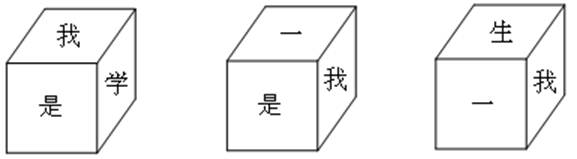
\includegraphics[width=6cm]{7NJ01-01-20190803-15.jpg}
\end{center}

\xx
{“生”和“一”}
{“初”和“生”}
{“初”和“一”}
{“生”和“初”}   


\end{onlyproblem}%
\begin{onlysolution}%
\begin{solution}%%
A
\end{solution}%
\end{onlysolution}%
\end{defproblem}



\begin{defproblem}{7NJ-02-09}%
\begin{onlyproblem}%
一个小立方块的六面分别标有字母A,B,C,D,E,F,如图是从三个不同方向看到的情形,则A,B,E的相对面分别是(    ) 
\begin{center}
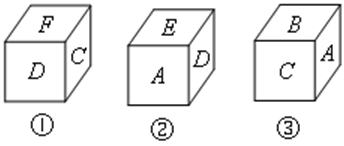
\includegraphics[width=5cm]{7NJ01-01-20190803-16.jpg}
\end{center}

\xx
{E,D,F}
{E,F,D}
{F,D,E}
{F,D,C}


\end{onlyproblem}%
\begin{onlysolution}%
\begin{solution}%%
D
\end{solution}%
\end{onlysolution}%
\end{defproblem}




\begin{defproblem}{7NJ-02-10}%
\begin{onlyproblem}%
一个正方体六个面上分别写着六个连续的整数,且每组相对面上的两个数之和相等,如图所示,你能看到的数为3,6,7,则六个整数的和为(    ) 
\begin{center}
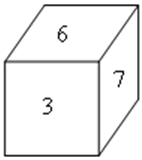
\includegraphics[width=1.5cm]{7NJ01-01-20190804-03}
\end{center}

\xx
{27}
{28}
{33}
{34}

\end{onlyproblem}%
\begin{onlysolution}%
\begin{solution}%%
C. 
能看到的三个整数是3,6,7,由于是六个连续的整数, 由题可知其中的五个数字是3,4,5,6,7, 所以第六个数字可能是2或者8, 如果是2的话,根据每组相对面上的两个数之和相等,那么3与6相对, 而图中3和6是相邻面,因此第六个数字只能是8, 此时3与8相对,4与7相对,5与6相对, 满足题中的条件,所以六个整数的和是$3+4+5+6+7+8=33$.三颗星知识点:正方体的表面展开图——相邻面、相对面
\end{solution}%
\end{onlysolution}%
\end{defproblem}




\begin{defproblem}{7NJ-02-11}%
\begin{onlyproblem}%
已知一不透明的正方体的六个面上分别写着1至6六个数字,如图是我们能看到的三种情况,那么2和4的对面数字分别是(    ) 
\begin{center}
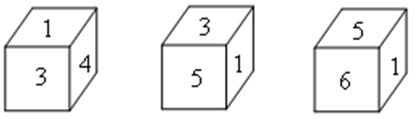
\includegraphics[width=6cm]{7NJ01-01-20190804-27}
\end{center}

\xx
{1, 6}
{3, 6}
{1, 5}
{3, 5}

\end{onlyproblem}%
\begin{onlysolution}%
\begin{solution}%%
C. 
解题思路: 正方体6个面中,每一个面和四个面相邻,和一个面相对. ①首先找图中出现次数最多的,是“1”,从图中的三个正方体可以看到 “1”和“3”,“4”,“5”,“6”相邻,所以“1”的相对面是“2”. ②接下来看“3”或“5”,不妨先看“3”,在剩下的四个面中, “3”和“4”,“5”相邻,所以“3”的相对面是“6”; ③剩余的“4”和“5”是相对面. 所以“2”和“4”的相对面分别是“1”和“5”. 故选C. 
三颗星知识点:正方体的表面展开图——相邻面、相对面  
\end{solution}%
\end{onlysolution}%
\end{defproblem}



\begin{defproblem}{7NJ-02-12}%
\begin{onlyproblem}%
有一正方体,六个面上分别写有数字1,2,3,4,5,6,有三个人从不同的角度观察的结果如图所示.如果记6的对面数字为a,2的对面数字为b,那么a+b的值为(    )
\begin{center}
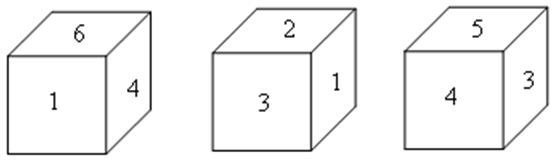
\includegraphics[width=6cm]{7NJ01-01-20190804-28}
\end{center}

\xx
{3}
{7}
{8}
{11}

\end{onlyproblem}%
\begin{onlysolution}%
\begin{solution}%%
B. 
解题思路: 本题通过相邻面确定相对面,正方体的每一个面与4个面相邻,1个面相对. 比如本题,先找出现次数较多的,不妨先从数字1开始:
\begin{center}
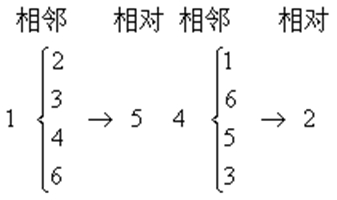
\includegraphics[width=6cm]{7NJ01-01-20190804-29}
\end{center}
 所以:1与5相对,4与2相对,3与6相对, 所以$a=3$,$b=4$,那么$a+b=3+4=7$. 故选B.  
\end{solution}%
\end{onlysolution}%
\end{defproblem}






